\section{Versuchsbeschreibung}
\label{section:Versuchsbeschreibung}
Der Prüfstand hat als Herzstück ein automatisiertes Brennstoffzellensystem.
Die Brennstoffzelle des Systems ist ein 47-zelliges PEM-Stack.
An den Stack sind über einen Laderegler zwei 12 V-Batterien, welche zu einem 24 V-Pufferspeicher verschaltet sind, angeschlossen.
Der Speicher ist, zum Ausgleichen eventueller Lastextrema durch Laden oder Entladen, parallel verschaltet.
Des Weiteren ist an das Brennstoffzellensystem eine elektronische Last angeschlossen,
welche als DC-Verbraucher fungiert und an welche die benötigten Arbeitspunkte eingestellt werden können.
Die Wasserstoffzufuhr ist mittels Drehhahn an der Wand einzustellen und kann
zusätzlich auf einem Volumenstrommesser in $\frac{Nl}{min}$ abgelesen werden.
Über eine Control-Unit ist das Brennstoffzellensystem auch an den Computer angeschlossen,
dieser gibt Stacktemperatur, -strom, -spannung und -leistung aus. Ebenfalls wird
damit der periphere Verbrauch durch den Kompressor und die Kühlung in \% ausgegeben.
Für die Messung von Batteriestrom- und -spannung werden zwei Multimeter an die Batterie angeschlossen.\\
Der Versuchsaufbau ist in \autoref{fig:Aufbau} dargestellt.
\begin{figure}[H]
    \centering
    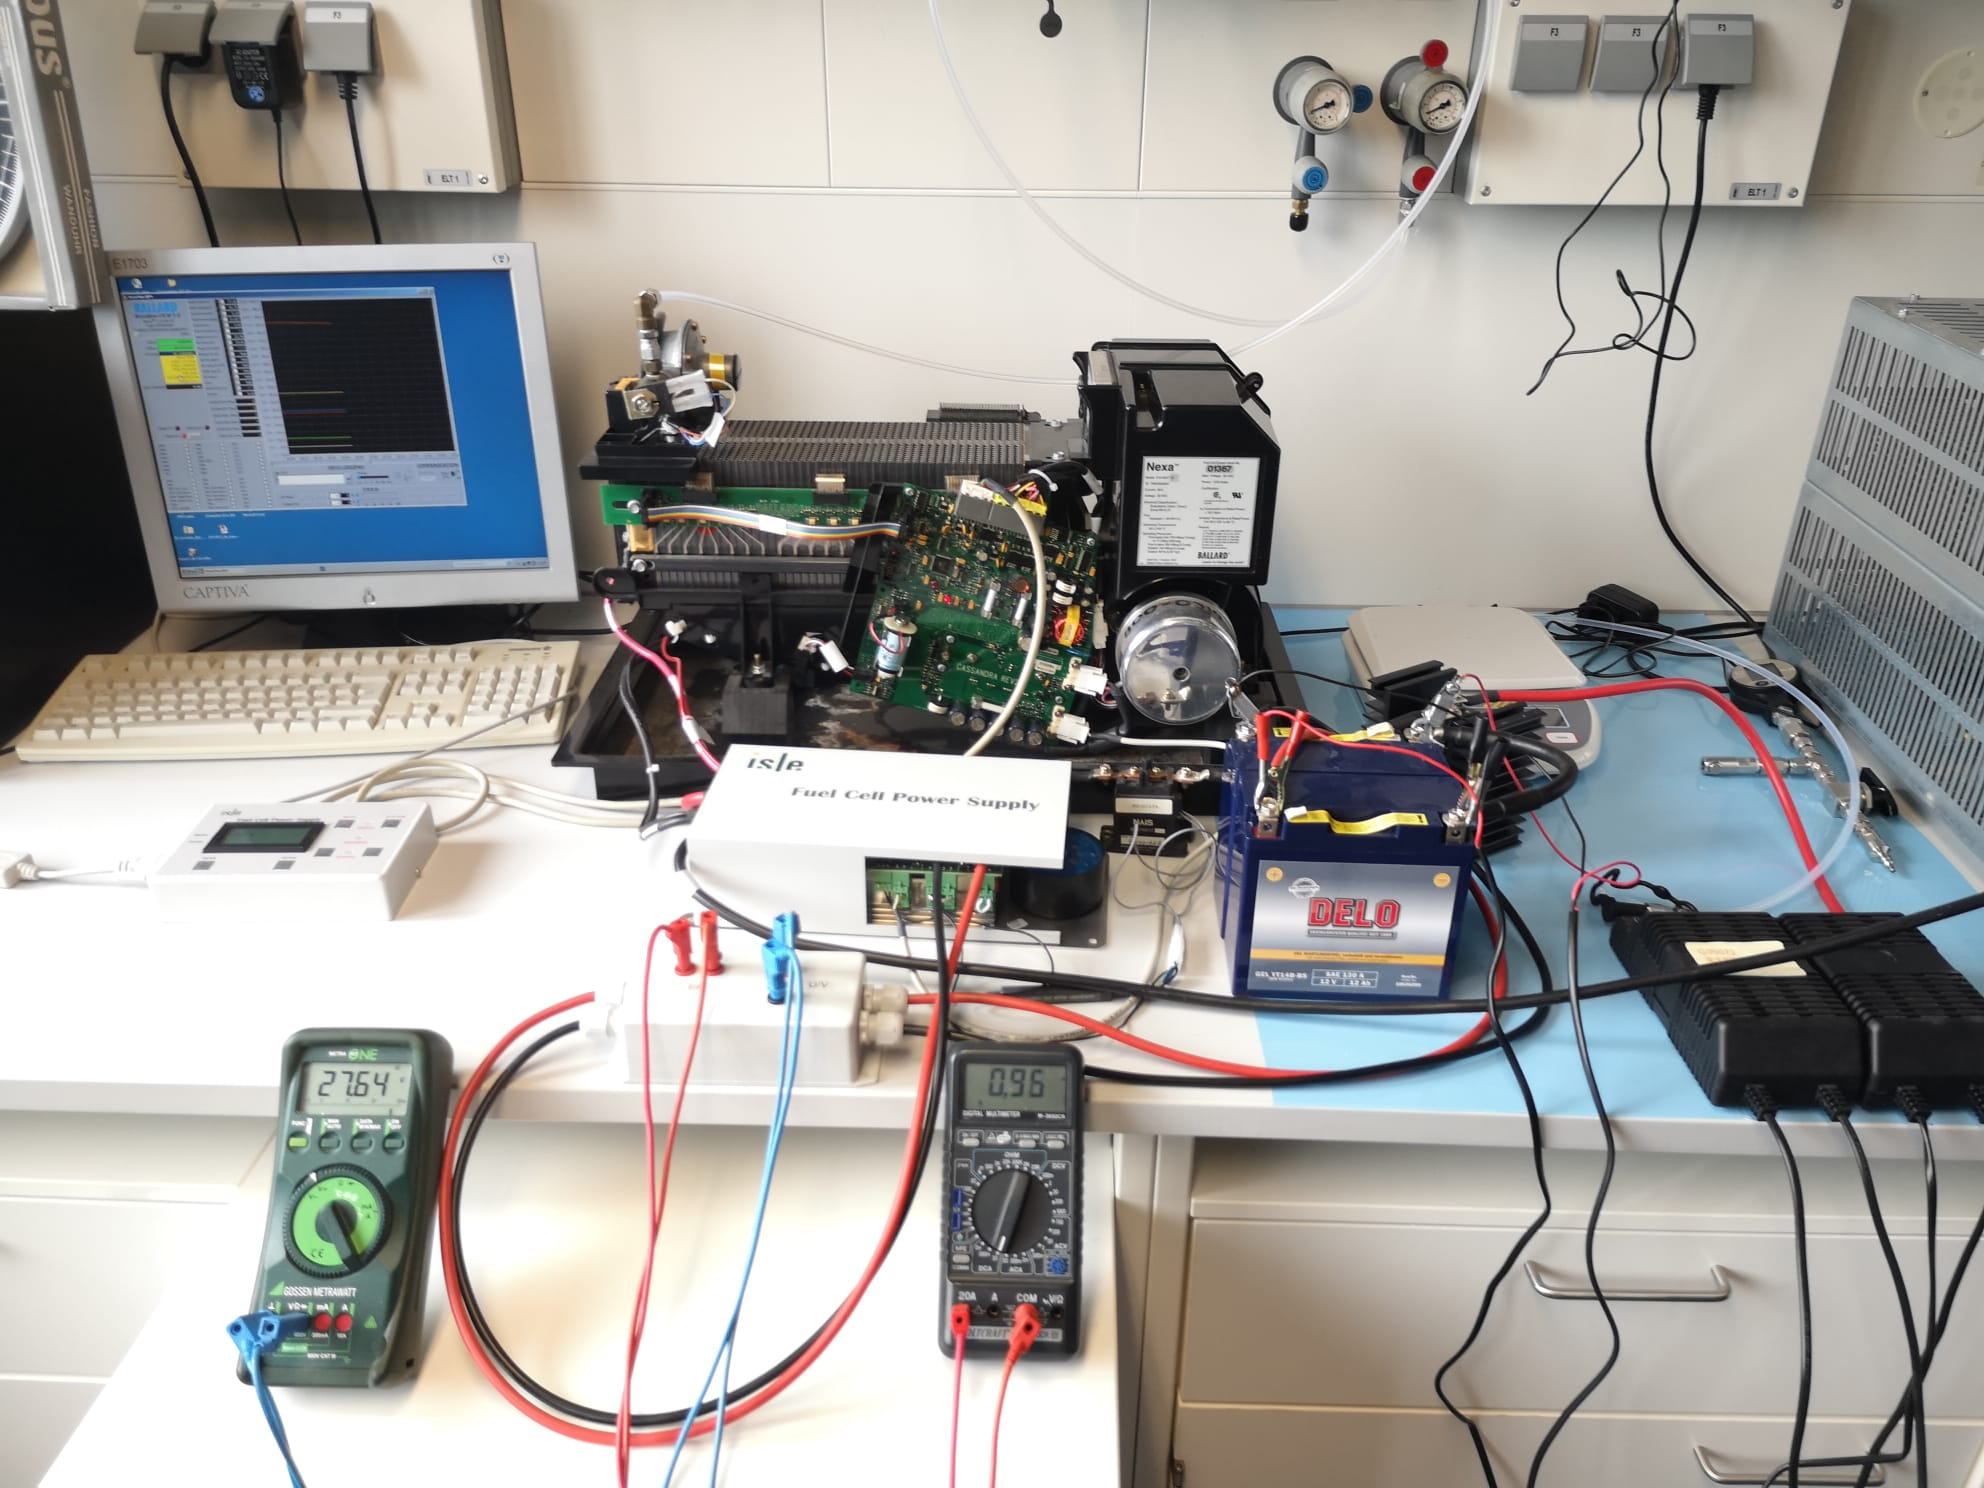
\includegraphics[width=\textwidth]{Abbildungen/Aufbau-Gesamt.jpg}
    \caption{Versuchsaufbau}
    \label{fig:Aufbau}
\end{figure}